\documentclass[SDSUThesis.tex]{subfiles} 
\begin{document}

% new section
\section{CASE STUDY: SCORING AN SDO OF A LARGE FINANCIAL INSTITUTION}

    Data has been collected from the software development processes of
    an SDO within a large financial institution\footnote{All the raw data 
    files are available at \cite{Swanstrom2015}}.
    The data collection was from 2007 to January 2015. Only 4 elements had available
    data, and not all elements had data available for the entire time period.  The
    elements to be used are: quality, availability, schedule, and requirements.
    CRI is still effective when not all data is available.
    The overall CRI score will then be a 
    weighted average of the available elements. 
    This section will serve as a guide to preparing the CRI score
    based upon the available data.  

    After the data has been collected, the raw data can be stored in the SDLC
    if desired.  Then scores for each of the 4 elements can be calculated.
    For this example, the value of $k$ will be 100 and the time
    frequency will be monthly.  Thus, scores will fall
    in the range $[-100,100]$.  Also, equal weighting is applied to 
    all elements and all Project IDs, Application IDs, and System IDs.
    
    \subsection{QUALITY}
        The first step to dealing with the quality data is a quick
        analysis of the data.  Table \ref{tab:quality_desc} provides
        some descriptive statistics for the quality data.  Testing hours
        were not captured, but they are optional, so the analysis can 
        continue.
        
        
        \begin{longtable}{@{}l rr rrr}
            \toprule%
             \centering%
             {\bfseries Column}
             & {\bfseries Min}
             & {\bfseries Max}
             & {\bfseries Median}
             & {\bfseries Mean}
             & {\bfseries Variance} \\
            
            \cmidrule[0.2pt](r{0.125em}){1-1}%
            \cmidrule[0.2pt](lr{0.125em}){2-2}%
            \cmidrule[0.2pt](l{0.125em}){3-3}%
            \cmidrule[0.2pt](l{0.125em}){4-4}%
            \cmidrule[0.2pt](l{0.125em}){5-5}%
            \cmidrule[0.2pt](l{0.125em}){6-6}%
            % \midrule
            \endhead
            
            Development Effort & 0 & 26937 & 300 & 1637 & 18383464 \\
            \myrowcolour%
            Testing Effort & NA & NA & NA & NA  & NA\\
            SIT Defects & 0 & 1106 & 1 & 45.86 & 24528 \\
            \myrowcolour%
            UAT Defects & 0 & 277 & 0 & 10.28 & 1306 \\
            PROD Defects & 0 & 1216 & 5 & 51.5 & 20311 \\
            
            \bottomrule
            
            \multicolumn{6}{c}{985 obs. from 23 Application IDs from 2007 to 2015} \\
            
            \caption{QUALITY DATA DESCRIPTIVE STATISTICS}
            \label{tab:quality_desc}
        \end{longtable}
        
        Notice, the data for quality goes from October 2007 to January 2015
        and contains 985 observations.
        This is important because historical data can be used to create the
        baseline quality function.  All quality for the years 2007 through 
        the end of 2013
        will be used as historical data for the purposes of creating
        the baseline quality function.  Once the historical data is separated,
        it results in 799 observations to be used for creating the baseline
        quality function.  Figure \ref{fig:quality-plots1} shows scatterplots
        of PROD\_DFTS versus the independent variables of DEV\_EFF, SIT\_DFTS,
        and UAT\_DFTS.  It can be seen that some correlations exist between
        the variables.
        
        \begin{figure}[htb]
            \centering
            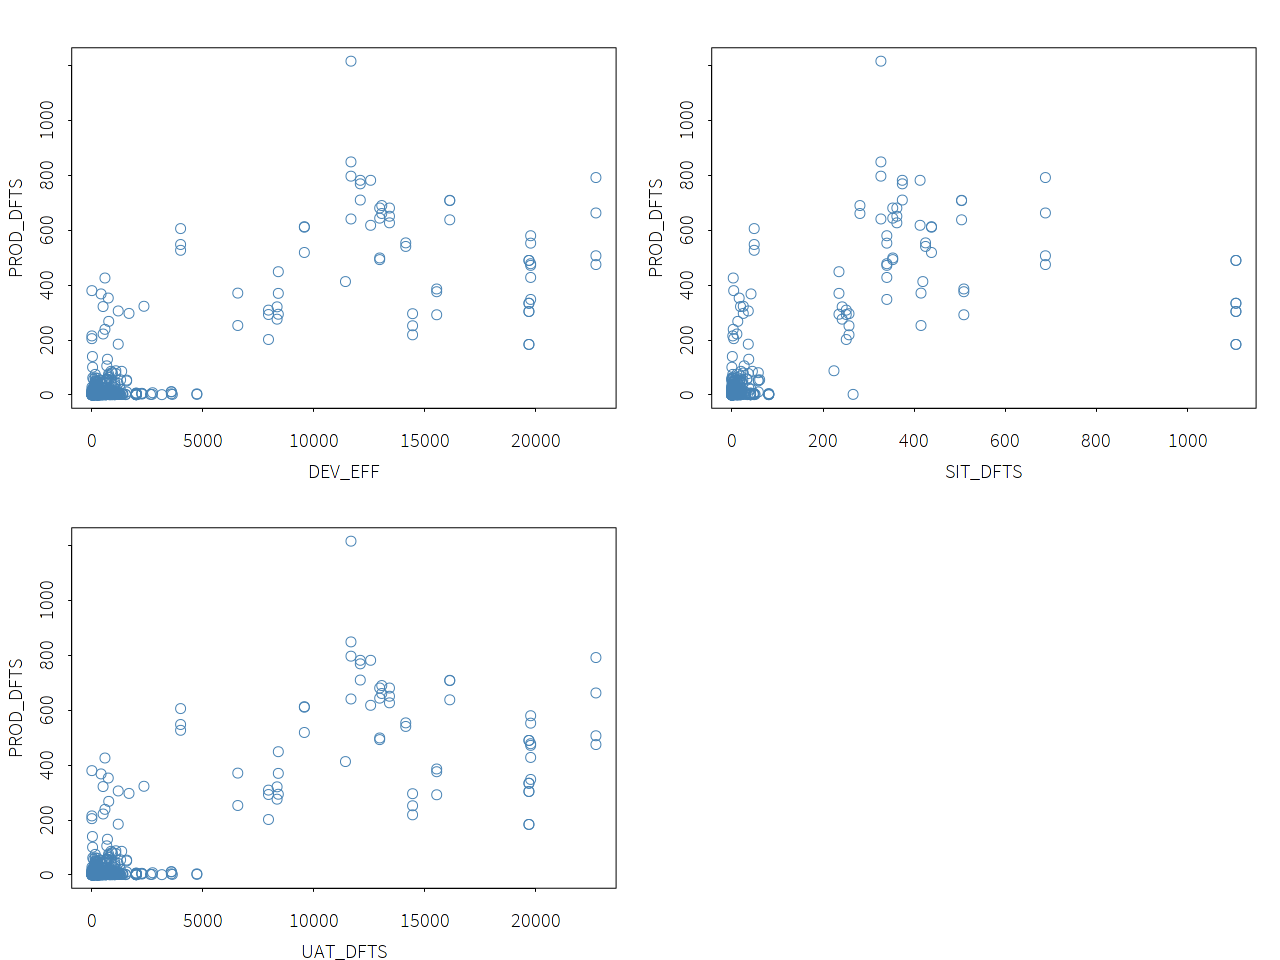
\includegraphics[scale=.25]{images/quality_plots1.png}
            \caption{QUALITY DATA PLOTS: DEPENDENT VS. INDEPENDENT VARIABLES}
            \label{fig:quality-plots1}
        \end{figure}
        
        Figure \ref{fig:quality-plots1} also shows the presence of a possible outlier
        with 1216 PROD\_DFTS.  That data point is dropped for the remaining analysis.
        At this point, a simple linear regression model can be fit to the remaining
        798 observations. At this point, no transformations have been performed
        on the data.  The linear regression model yields all 3 independent
        variables as significant and an overall $R^2 = .72$.  The source
        code and some further analysis can be found in Appendix 
        \ref{app:quality-history}. It appears to 
        be a good fit and thus all Application IDs will have the same baseline
        quality function.  Therefore, $f$ does not need a subscript, and $f$
        can be seen below.
        
        \[
            f = 5.92+ 0.035 \cdot DEV\_EFF - 0.36 \cdot SIT\_DFTS + 1.05 \cdot UAT\_DFTS
        \]
        
        Now that $f$ has been determined, the quality scores for each
        application can be calculated for all the months beyond 2013.
        Appendix \ref{src:quality} provides the necessary R code to
        perform the calculations.  Figure \ref{fig:quality-scores} shows
        the quality scores for 2014 and beyond.  As can be seen, the
        scores are greatly above expectations.  That is an indication
        of improved quality over historical performance.
        
        \begin{figure}[htb]
            \centering
            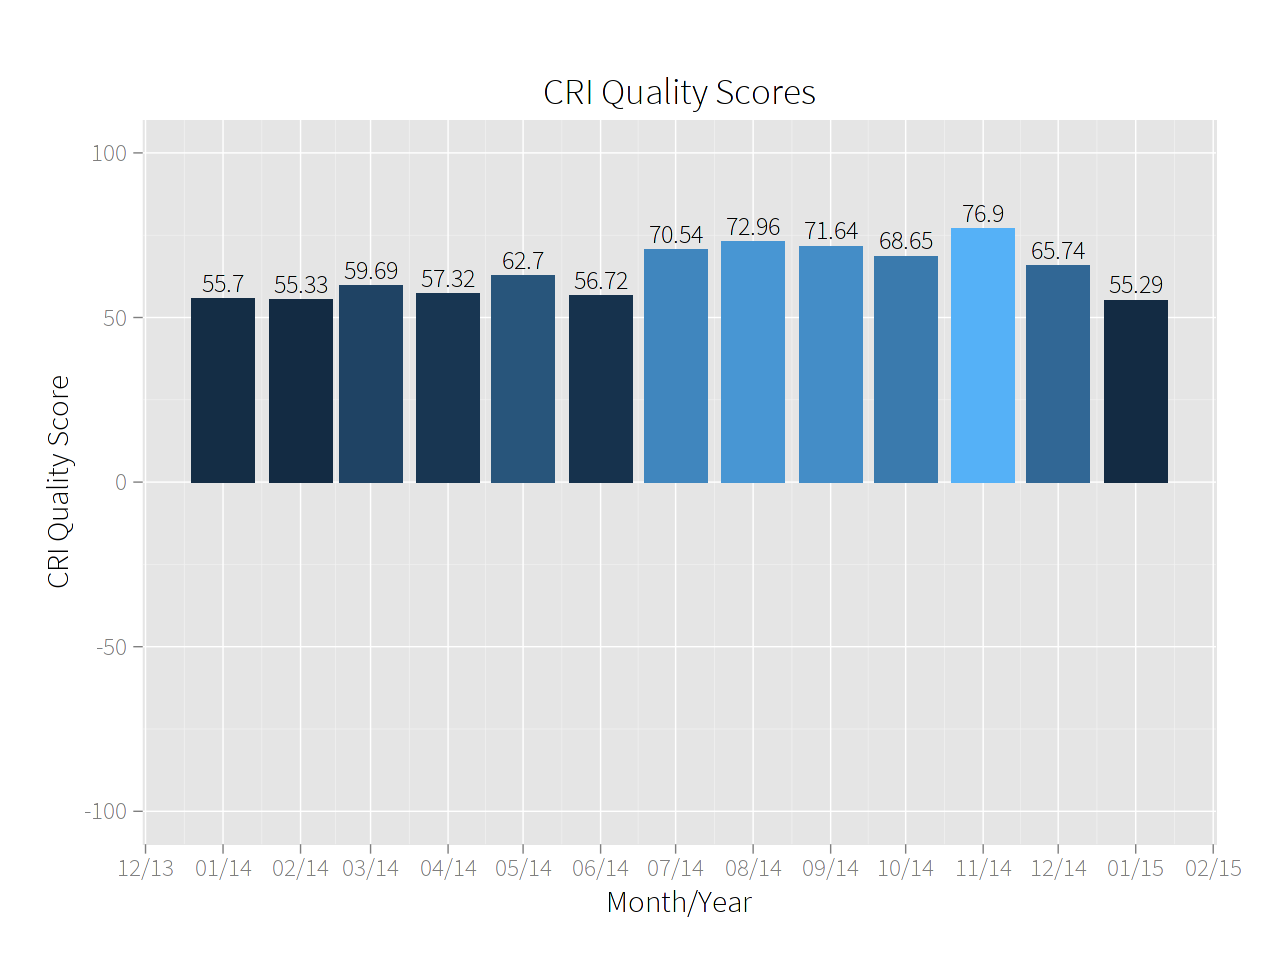
\includegraphics[scale=.3]{images/quality_scores.png}
            \caption{CRI QUALITY SCORES}
            \label{fig:quality-scores}
        \end{figure}
        
    \subsection{AVAILABILITY}
        For the availability data,
        some descriptive statistics can be seen in 
        Table \ref{tab:availability_desc}.  The percent uptime
        was previously calculated for this data so uptime, scheduled downtime,
        and unscheduled downtime are not needed.  Availability
        does not rely upon analysis of historical data since
        a known upper and lower bound exist, 1 and 0 respectively.
        
        The numbers in Table \ref{tab:availability_desc} indicate
        the values are very near 1.  This is expected as SDOs
        set SLA uptime values near 1, and even strive to meet
        an uptime of 1.  An uptime of 1 means the system was
        available the entire time period.  Thus numbers for uptime
        near 1 are highly desirable for an SDO expecting
        to score well for availability.
        
        \begin{longtable}{@{}l rr rrr}
            \toprule%
             \centering%
             {\bfseries Column}
             & {\bfseries Min}
             & {\bfseries Max}
             & {\bfseries Median}
             & {\bfseries Mean}
             & {\bfseries Variance} \\
            
            \cmidrule[0.2pt](r{0.125em}){1-1}%
            \cmidrule[0.2pt](lr{0.125em}){2-2}%
            \cmidrule[0.2pt](l{0.125em}){3-3}%
            \cmidrule[0.2pt](l{0.125em}){4-4}%
            \cmidrule[0.2pt](l{0.125em}){5-5}%
            \cmidrule[0.2pt](l{0.125em}){6-6}%
            % \midrule
            \endhead
            
            Percent Uptime & 0 & 1.0 & 1.0 & 0.9745 & 0.023 \\
            \myrowcolour%
            Expected Percent Uptime & 0.93 & 1.0 & 0.98 & 0.9769  & 0.977\\
            
            \bottomrule
            
            \multicolumn{6}{c}{7522 obs. from 83 Application IDs from 2008 to 2015} \\
            
            \caption{AVAILABILITY DATA DESCRIPTIVE STATISTICS}
            \label{tab:availability_desc}
        \end{longtable}
        
        Since percent uptime has already been calculated and no historical
        analysis needs to be performed, the calculation of the scores
        can be performed. 
        R code to compute the CRI availability scores can be found in Appendix
        \ref{src:availability}. Figure \ref{fig:availability-scores} displays
        the CRI availability scores.  
        
        \begin{figure}[hb]
            \centering
            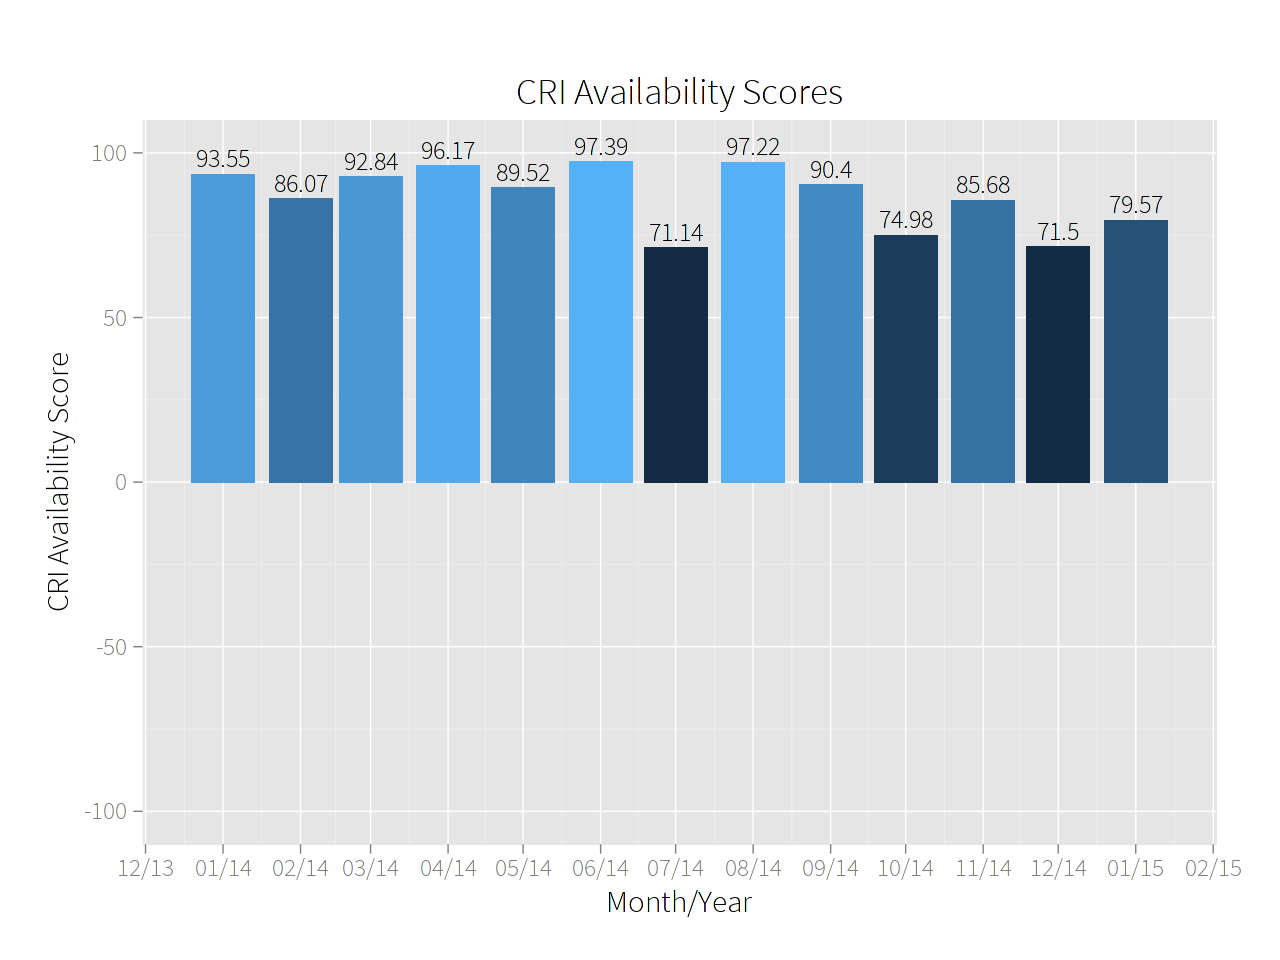
\includegraphics[scale=.3]{images/availability_scores.png}
            \caption{CRI AVAILABILITY SCORES}
            \label{fig:availability-scores}
        \end{figure}
        
        As can be seen in Figure  \ref{fig:availability-scores}
        the scores are all above 70 which
        is good from a performance standpoint, but it might be an
        indication that the expected uptimes could be raised.  If expected
        uptimes are consistently being exceeded, some consideration should
        be given to increase the expected uptimes.  This shows that
        organizations, or at least this particular organization, are getting
        very good at keeping computer systems available.  Therefore,
        SLAs need to be adjusted to properly reflect the better performance.
        
        
    \subsection{SCHEDULE}
        Figure \ref{tab:schedule_desc} displays some descriptive statistics
        for the schedule data.  Since the data is mostly dates, the 
        descriptive statistics are limited, so extra values were
        added to the table after removing 4 outliers.  The new values
        in the table are: Schedule Duration (Scheduled Finish - Scheduled Start),
        Difference (Actual Finish - Schedule Finish), and 
        $\Delta$ ($\frac{\text{Difference}}{\text{Schedule Duration}}$ ).
    
        \begin{longtable}{@{}l rr rrr}
            \toprule%
             \centering%
             {\bfseries Column}
             & {\bfseries Min}
             & {\bfseries Max}
             & {\bfseries Median}
             & {\bfseries Mean} \\
            
            \cmidrule[0.2pt](r{0.125em}){1-1}%
            \cmidrule[0.2pt](lr{0.125em}){2-2}%
            \cmidrule[0.2pt](l{0.125em}){3-3}%
            \cmidrule[0.2pt](l{0.125em}){4-4}%
            \cmidrule[0.2pt](l{0.125em}){5-5}%
            % \midrule
            \endhead
            
            Scheduled Start & 2013-06-23 & 2015-01-24 & 2014-03-17 & 2014-04-01 \\
            \myrowcolour%
            Scheduled Finish & 2014-01-31 & 2015-01-25 & 2014-08-08 & 2014-08-02 \\
            Actual Start & 2013-01-07 & 2014-10-17 & 2014-01-15  & 2014-02-10 \\
            \myrowcolour%
            Actual Finish & 2014-02-20 & 2014-12-31 & 2014-08-31 & 2014-08-11 \\
            Schedule Duration & 8 & 480 & 92 & 137.7 \\
            \myrowcolour%
            Difference & -283 & 149 & 0.0 & -8.919 \\
            $\Delta$ & -4.75 & 0.6564 & 0.0 & -0.2641 \\
            
            \bottomrule
            
            \multicolumn{5}{c}{41 obs. from 40 Project IDs from mid 2013 to 2015} \\
            
            \caption{SCHEDULE DATA DESCRIPTIVE STATISTICS}
            \label{tab:schedule_desc}
        \end{longtable}
        
        The first task with the schedule data is fitting the data to 
        a distribution.  Figure \ref{fig:schedule-hist} shows
        a plot of the histogram of the $\Delta$s and a
        Cauchy curve with location = 0.0 and scale = 0.057.  The Cauchy
        distribution appears to be a good fit.  
        
        \begin{figure}[htb]
            \centering
            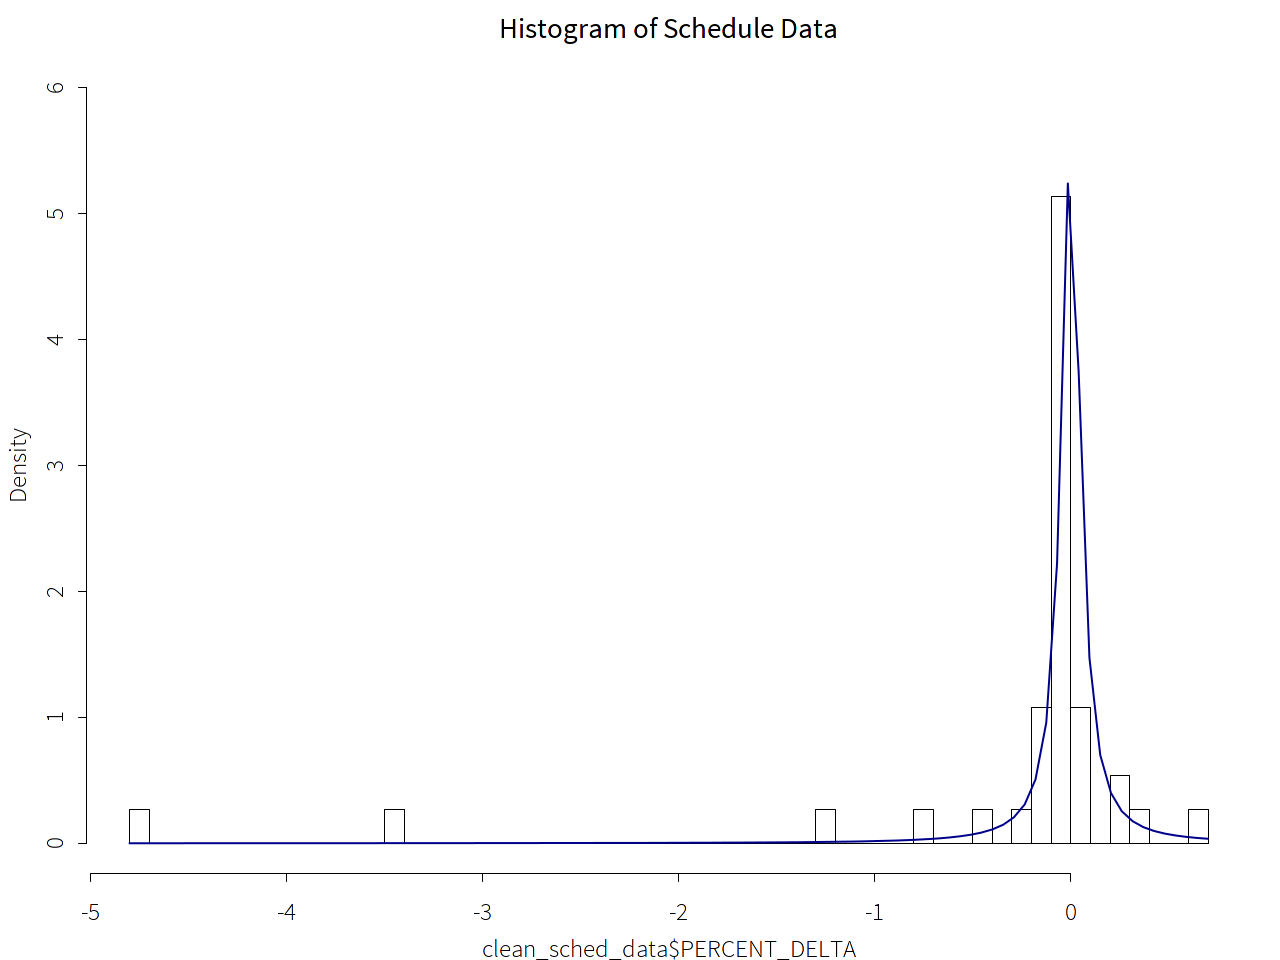
\includegraphics[scale=.25]{images/schedule_hist.png}
            \caption{SCHEDULE DATA HISTOGRAM WITH CAUCHY}
            \label{fig:schedule-hist}
        \end{figure}
        
        Now that the distribution has been identified, the next step
        is determining the CDF
        for the distribution.  For Cauchy, the general CDF is 
        given as follows.
        \[
            CDF(x) = \frac{1}{\pi}\arctan{\frac{x-x_0}{\gamma}} + \frac{1}{2}
        \]
        where 
        \begin{itemize}
            \item $x_0$ is the location
            \item $\gamma$ is the scale
        \end{itemize}
        
        Referencing Equation \ref{eq:CDF}, the schedule formula
        for individual project IDs becomes.
        \[
           S_{4_i} = \frac{200}{\pi}\arctan{\left(\frac{\Delta_i}{0.057} \right)} 
        \]
        
        The CRI schedule scores can be seen in Figure \ref{fig:schedule-scores}.
        These scores appear more erratic than the other elements.
        This difference is due to the small number of releases every month.
        
        \begin{figure}[htb]
            \centering
            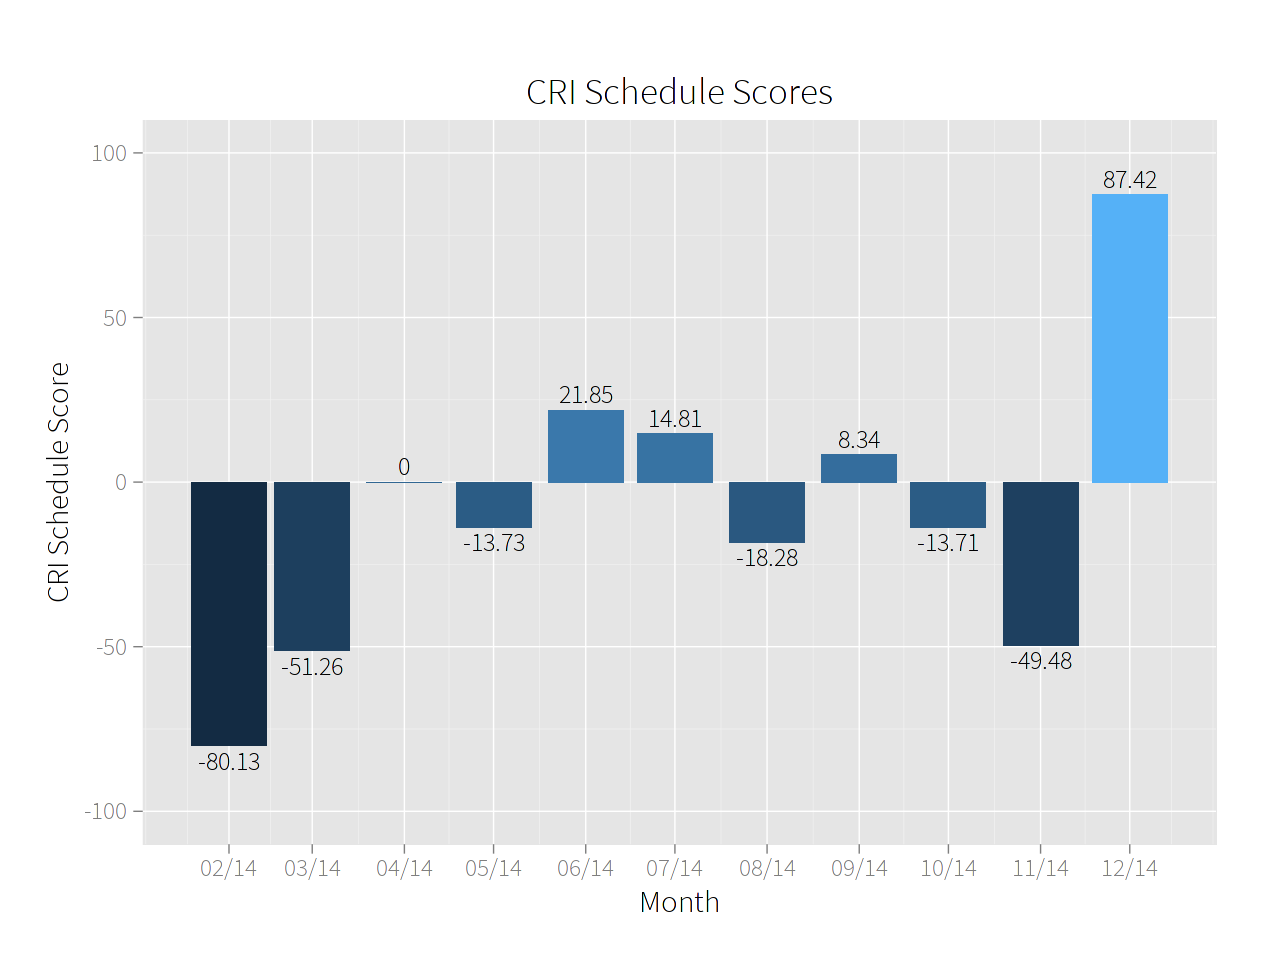
\includegraphics[scale=.3]{images/schedule_scores.png}
            \caption{CRI SCHEDULE SCORES}
            \label{fig:schedule-scores}
        \end{figure}
        
        
    \subsection{REQUIREMENTS}
    \label{sec:case-req}
        The data for requirements is actually counts of story points
        instead of requirements.  That is because story points
        are a better choice for counting, since they are more
        uniform in size than raw requirements.  Also, the data
        contained 15 rows of data with a 0 for the number of
        scheduled requirements.  Those 15 rows were removed.
        Table \ref{tab:requirements_desc} shows some descriptive
        statistics for the remaining rows. A histogram for the
        data can be seen in Appendix \ref{app:requirements-hist}.
        
        \begin{longtable}{@{}l rr rrr}
            \toprule%
             \centering%
             {\bfseries Column}
             & {\bfseries Min}
             & {\bfseries Max}
             & {\bfseries Median}
             & {\bfseries Mean}
             & {\bfseries Variance} \\
            
            \cmidrule[0.2pt](r{0.125em}){1-1}%
            \cmidrule[0.2pt](lr{0.125em}){2-2}%
            \cmidrule[0.2pt](l{0.125em}){3-3}%
            \cmidrule[0.2pt](l{0.125em}){4-4}%
            \cmidrule[0.2pt](l{0.125em}){5-5}%
            \cmidrule[0.2pt](l{0.125em}){6-6}%
            % \midrule
            \endhead
            
            Scheduled Requirements & 0.5 & 1248 & 75.5 & 136.9 & 31243.89 \\
            \myrowcolour%
            Actual Requirements & 0 & 1247 & 58 & 123.8 & 30844.75 \\
            $\frac{Actual Requirements}{Scheduled Requirements}$ & 0 & 1.2364 & 1.0 & 0.8515 & 0.05 \\
            
            \bottomrule
            
            \multicolumn{6}{c}{461 obs. from 402 Project IDs from 2010 to 2015} \\
            
            \caption{REQUIREMENTS DATA DESCRIPTIVE STATISTICS}
            \label{tab:requirements_desc}
        \end{longtable}
        
        The multiplier $b$ is set to 1 because none of the historical performance
        ever exceeded 25\% more requirements than scheduled. Thus the upper
        bound is the number of schedule requirements plus $b=1$ times
        the number of scheduled requirements, for an upper bound of twice
        the scheduled requirements.
        
        \begin{figure}[htb]
            \centering
            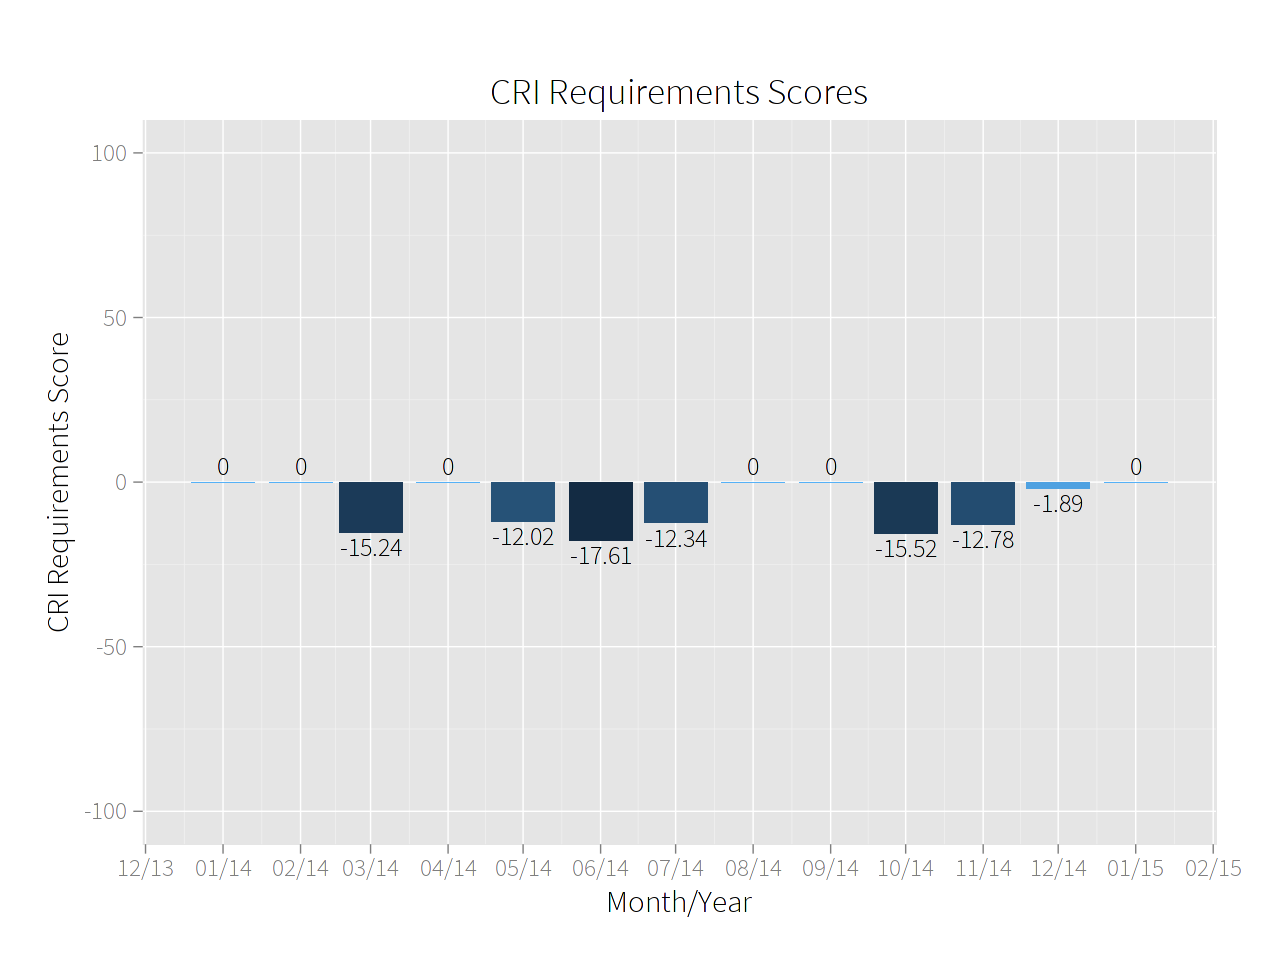
\includegraphics[scale=.3]{images/requirements_scores.png}
            \caption{CRI REQUIREMENTS SCORES}
            \label{fig:requirements-scores}
        \end{figure}
        
        Figure \ref{fig:requirements-scores} displays the CRI requirements
        scores. The scores are as expected considering the histogram. Many
        of the projects meet the requirements exactly, and when the requirements
        are not met, it is usually by a small number.
        Thus the scores are all 0 or slightly below.
        
    \subsection{OVERALL}
        Now it is time to combine the scores for the overall CRI.
        Schedule does not have scores for January 2014 or January 2015.
        Presumably, that is because the SDO within the large financial institution
        does not schedule projects to be completed in January. Much of the work
        would need to be completed over Christmas and New Year's Day, but many
        workers take personal time off of work during that time.  Thus some
        organizations will schedule appropriately.  CRI is well suited to
        handle this problem.  Just perform a weighted average over the
        applicable elements.  In this case study, the weights are all equal,
        so CRI is just a straight average.  
        
        \begin{figure}[htb]
            \centering
            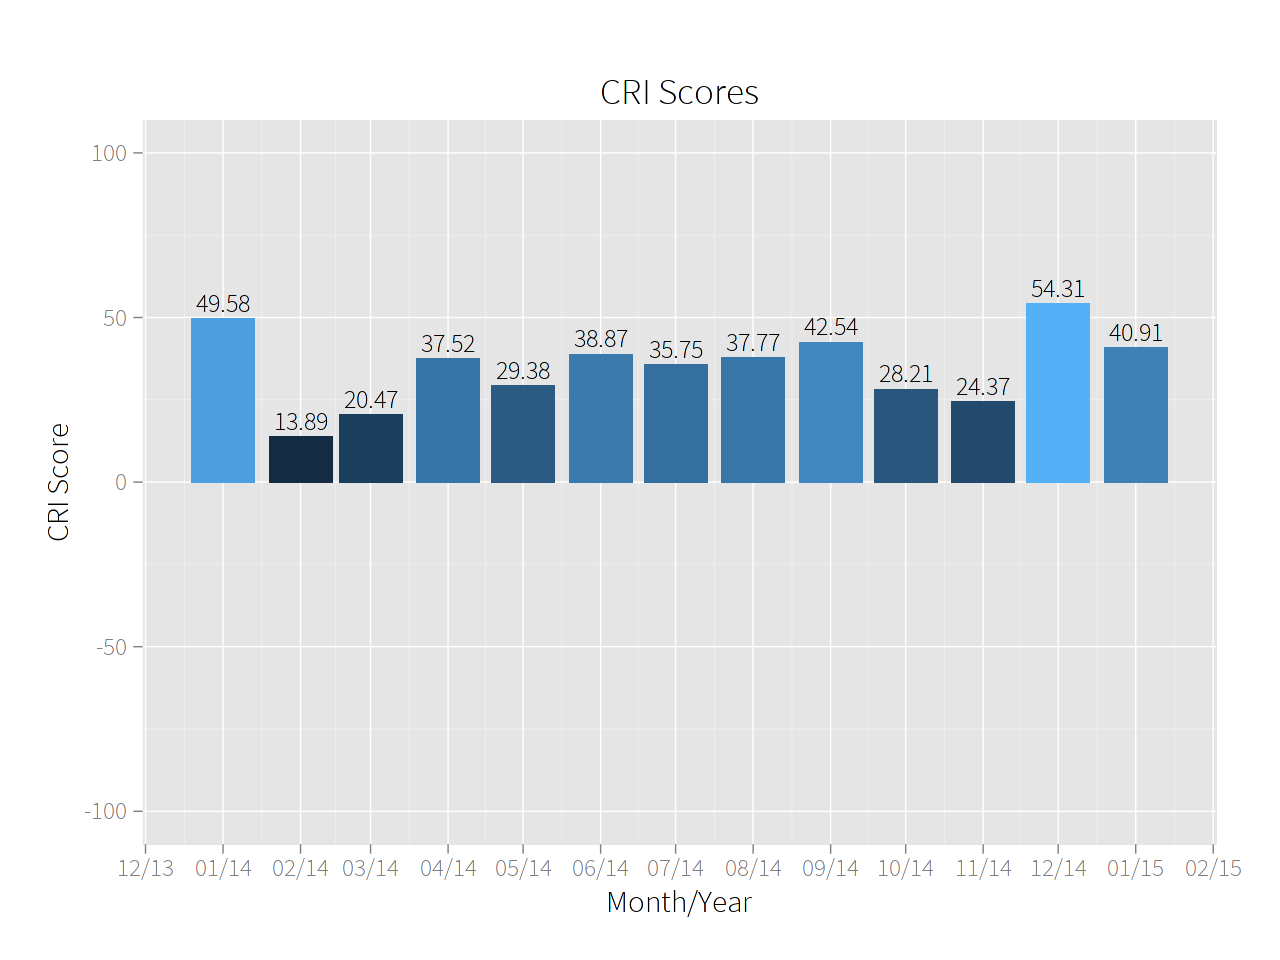
\includegraphics[scale=.3]{images/cri_scores.png}
            \caption{CRI SCORES}
            \label{fig:cri-scores}
        \end{figure}
        
        Figure \ref{fig:cri-scores}
        displays the CRI scores as computed with the source code
        from Appendix \ref{src:overall}.  The scores are all above 0, so this
        financial institution has performed consistently better
        than expected.  
        
    \subsection{SENSITIVITY AND CORRELATION}
        
        To check the sensitivity of the CRI formula, the first method
        from Section \ref{sec:sensitivity} is used.  Small random
        values were added to the input values of the formulas. 
        Then the new values were used to calculated the element scores 
        at the respective Application ID or Project ID level.  Finally
        the new CRI element scores were compared with the previous
        scores from the unaltered data.  The goal is to show small
        changes in the input values result in small changes to the 
        CRI element score.  Figure \ref{fig:sensitivity} shows
        histograms of the new scores compared with the previous scores.
        None of the formulas exhibit too much sensitivity as the 
        histograms all indicate most of the score changes are small,
        as seen by the high peak of the histograms.  
        
        \begin{figure}[htb]
            \centering
            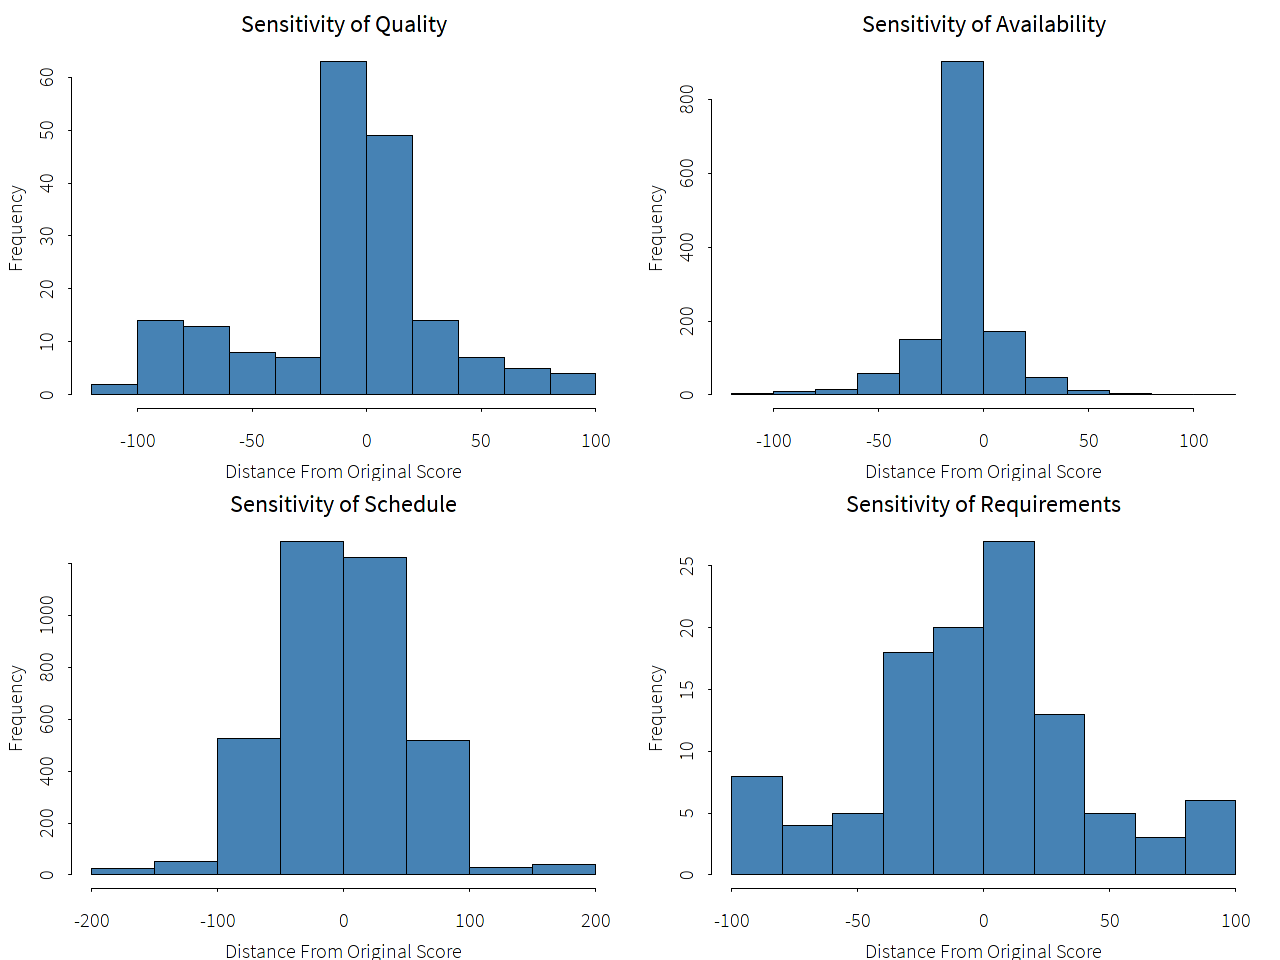
\includegraphics[scale=.3]{images/sensitivity.png}
            \caption{CRI SENSITIVITY ANALYSIS}
            \label{fig:sensitivity}
        \end{figure}
         
        The random values added were based on the standard 
        deviations of the values in the column.
        Quality and Requirements used the standard deviation of the
        matching Application ID or Project ID.  This slight difference
        is due to the wide variation of standard deviations between
        Application IDs for Quality and Project IDs for Requirements. 
        Table \ref{tab:sensitivity} shows the columns that were
        altered for each element.  
        
        \begin{longtable}{@{}l r}
            \toprule%
             \centering%
             {\bfseries CRI Element}
             & {\bfseries Columns Altered } \\
            
            \cmidrule[0.2pt](r{0.125em}){1-1}%
            \cmidrule[0.2pt](r{0.125em}){2-2}%
            % \midrule
            \endhead
            
            Quality  & Development Effort, SIT Defects, UAT Defects \\
            \myrowcolour%
            Availability & Percent Uptime \\
            Schedule &  $\frac{\text{Schedule Finish - Actual Finish}}
                    {\text{Scheduled Finish - Scheduled Start}}$ \\
            \myrowcolour%
            Requirements & Actual Requirements Released \\
            
            \bottomrule
            
            \caption{CRI SENSITIVITY ANALYSIS}
            \label{tab:sensitivity}
        \end{longtable}
        
        The columns were altered by adding
        random noise from a normal distribution with mean 0 and standard
        deviation as explained above.  The only exception to the normal
        distribution was for the schedule element.  The schedule element
        drew its noise from a Cauchy distribution with location and scale
        as defined when determining the distribution of the schedule data.
        That Cauchy distribution can be seen with the histogram in 
        Figure \ref{fig:schedule-hist}. 
        
        Figure \ref{fig:correlation_cri} shows a scatterplot matrix
        for the individual element scores.  No correlation appears
        to exist between any of the elements. The missing element,
        satisfaction, is the most likely element to exhibit correlation,
        so the 4 elements analyzed here remain independent.
        
        
        \begin{figure}[htb]
            \centering
            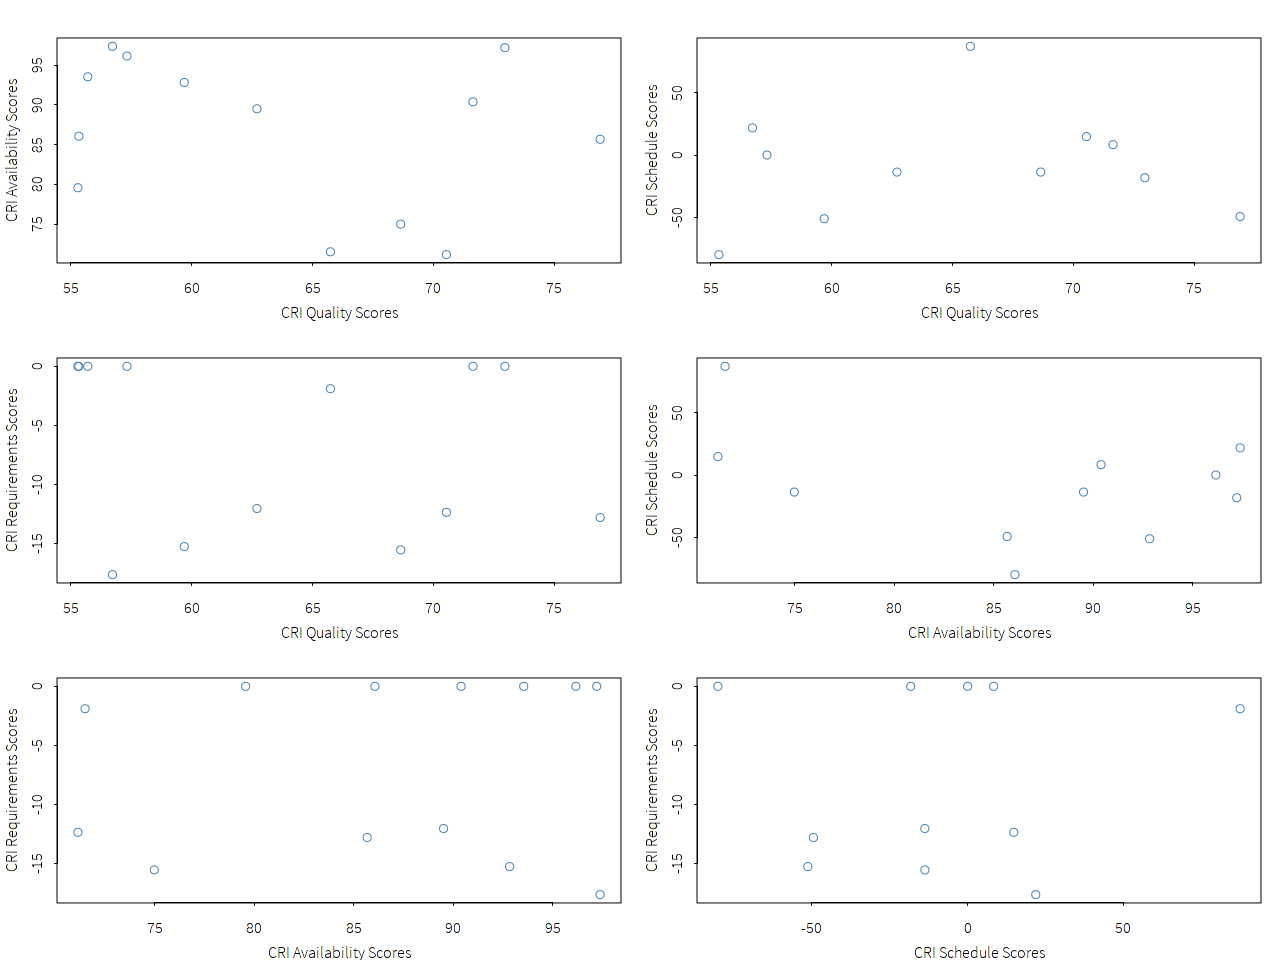
\includegraphics[scale=.3]{images/correlation.png}
            \caption{SCATTERPLOT MATRIX OF CRI ELEMENT SCORES}
            \label{fig:correlation_cri}
        \end{figure}
        

\end{document}